Формат *.deb --- расширение имён файлов <<бинарных>> пакетов для распространения и установки программного обеспечения в ОС проекта Debian и других, использующих систему управления пакетами dpkg. Пакеты Debian содержат исполняемые и конфигурационные файлы, номер версии формата, информацию об авторских правах, а также другую документацию, необходимую для установки программы из пакета.

Основные составляющие *.deb-пакета, необходимые для его создания:
\begin{itemize}
  \item control;
  \item md5sums;
  \item changelog;
  \item rules;
  \item README;
  \item conffiles;
  \item dirs;
  \item watch.
\end{itemize}

Control --- центральный файл пакета (обязательный), описывающего все основные свойства. Файл --- текстовый, состоящий из пар <<Атрибут: значение>>.

Md5sums --- содержит md5-хеши для всех файлов, кроме файлов, находящихся в каталоге DEBIAN/. Данный файл необязателен для deb-пакета, 
однако программы верификации пакетов считают пакеты, не содержащие этот файл, ошибочными. Может использоваться некоторыми программами администрирования системы для верификации изменений в файловой системе. Осуществляет контроль целостности файлов.

Changelog --- обязательный файл, его специальный формат описан в руководстве по политике Debian, раздел 4.4 <<debian/changelog>>. Этот формат используется программой dpkg и другими для получения информации о номере версии, редакции, разделе и срочности пакета.~\cite{deb_package_howto}

Rules --- используется для управления компиляцией пакета. 

README --- в этот файл записывается любая дополнительная информация, а также различия между программой из пакета Debian и исходной программой.

Conffiles --- Обычно пакеты содержат <<болванки>> конфигурационных файлов, например, размещаемых в /etc. Очевидно, что если конфигурационный файл в пакете обновляется, пользователь потеряет свой отредактированный конфигурационный файл. Эта проблема легко решается использованием папок типа <<config.d>>, содержимое которых включается в основной конфигурационный файл, заменяя собой повторяющиеся опции.~\cite{deb_man}

Dirs --- в этом файле указываются каталоги, которые необходимы для обычной установки (make install DESTDIR=..., вызываемая dh\_auto\_install), но которые автоматически не создаются. Обычно, это указывает на проблему в Makefile.

Watch --- формат файла watch описан в справочной странице uscan(1). Файл watch настраивает программу uscan (предоставляется пакетом devscripts) для слежения за сайтами, с которых вы скачали исходный код. Он также используется службой Debian для слежения за состоянием внешних источников (DEHS).~\cite{deb_package_howto}

Для решения данной  задачи было сделано:

\begin{itemize}
\item изучен *.deb формат, особенности файлов стандартов необходимых для создания данного пакета и установки его в операционные системы семейства Unix; 
\item изучены программные продукты для работы с данным форматом (dpkg, build-essential,  quilt, fakeroot, devscripts, debhelper и dh-make, lintian);
\item изучены особенности написания скриптов bash для операционных систем Unix;
\item ознакомление и изучение программы make, набора инструкцией Makefile и программной утилиты для QT C++ qmake;
\item углубленное изучение системы построения программного комплекса <<COEX>> и зависимых библиотек для компиляции данного программного комплекса;
\item создание двух программ bash-скриптов для формирования *.deb пакета и формирования changelog на основе истории коммитов системы контроля версий GIT;
\item тестирование на <<чистой>> операционной системе Linux Mint 17.2;
\item изучен формат набора макрорасширений системы компьютерной вёрстки LaTeX, личный отчет по групповому проектному обучению был оформлен согласно данному формату, и отдан документатору для редакции и включения в общий отчет.
\end{itemize}

\subsubsection{ Подробное рассмотрение набора bash-скриптов для формирования *.deb пакета и формирования changelog}

В начале программы с помощью скрипта build.sh компилируется проект и осуществляется сборка бинарного файла <<coex>>, а также динамических библиотек, используемых программным комплексом <<COEX>>. Исполняемые файлы плагинов данного проекта имеют формат *.so. 

В корне пакета создается папка <<DEBIAN>>. Эта папка содержит управляющую генерацией пакета информацию и не копируется на диск при установке пакета.
Также корневая папка пакета содержит будущий <<корень диска>>: при установке пакета все файлы (кроме папки <<debian>>) распаковываются в корень /. Поэтому бинарный файл должен лежать по пути относительно корня пакета <<usr/bin/coex>>, что и было сделано в скрипте create\_package.sh (рис.~\ref{cpcoex:cpcoex}). 

\begin{figure}[h!]
\center{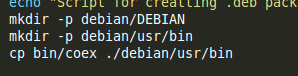
\includegraphics[width=0.5\linewidth]{cpcoex}}
\caption{Копирование основного бинарного файла проекта}
\label{cpcoex:cpcoex}
\end{figure}

Исполняемые файлы плагинов и программные библиотеки программного комплекса <<COEX>> представлены на рисунке~\ref{PluginsAndLibs:PluginsAndLibs}.

\begin{figure}[h!]
\center{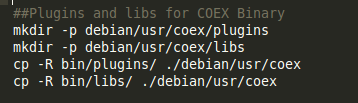
\includegraphics[width=0.6\linewidth]{PluginsAndLibs}}
\caption{Исполняемые файлы плагинов и программные библиотеки программного комплекса <<COEX>>}
\label{PluginsAndLibs:PluginsAndLibs}
\end{figure}

Установка иконки продукта нужна для графического интерфейса пользователя программного комплекса <<COEX>> (рис.~\ref{image:image}). Файл coex.desktop служит для запуска приложения, содержит основную информацию о программном комплексе <<COEX>> (рис.~\ref{Aplicatio:Aplicatio}).

\begin{figure}[h!]
\center{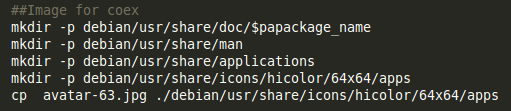
\includegraphics[width=0.6\linewidth]{image}}
\caption{ Иконка для GUI приложения <<COEX>> }
\label{image:image}
\end{figure}


\begin{figure}[h!]
\center{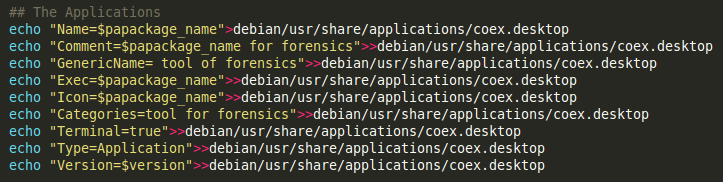
\includegraphics[width=0.6\linewidth]{Aplicatio}}
\caption{ Файл coex.desktop <<COEX>> }
\label{Aplicatio:Aplicatio}
\end{figure}

Лицензия на программный комплекс <<COEX>> защищает права разработчиков данного программного обеспечения. Руководство по использованию программного комплекса <<COEX>> находится в стадии разработки и будет содержать основные команды для использования программного комплекса <<COEX>>, информацию о плагинах и об особенностях работы с ними (рис.~\ref{LIcenzMan:LIcenzMan}).

\begin{figure}[h!]
\center{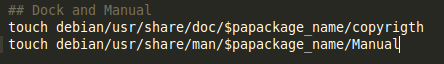
\includegraphics[width=0.6\linewidth]{LIcenzMan}}
\caption{ Лицензия и мануал по <<COEX>> }
\label{LIcenzMan:LIcenzMan}
\end{figure}

Файл control (рис.~\ref{control:control}) --- обязательный файл, в котором прописана версия программного комплекса <<COEX>>. Также указаны зависимости от библиотек, нужных для использования <<COEX>>.

\begin{figure}[h!]
\center{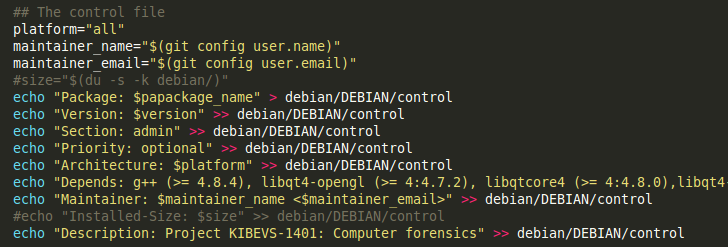
\includegraphics[width=0.8\linewidth]{control}}
\caption{ Файл control }
\label{control:control}
\end{figure}

Файл changelog (рис.~\ref{chengelog:chengelog}) --- в данном файле находятся сведения о всех изменениях программного комплекса <<COEX>> и версий пакета. Данный файл генерируется в отдельном скрипте gen\_change\_log.sh рисунок 10

\begin{figure}[h!]
\center{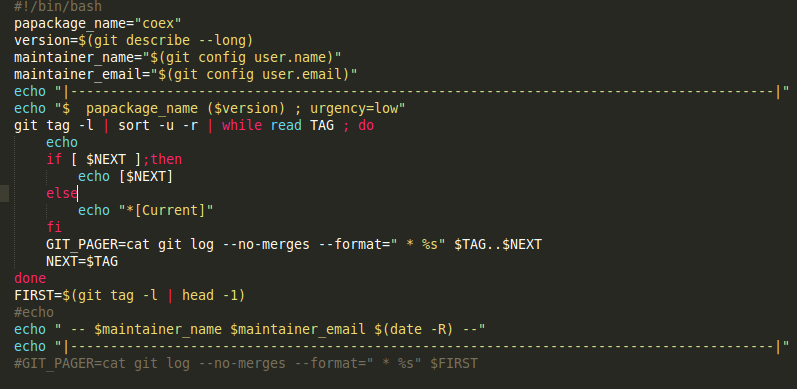
\includegraphics[width=0.8\linewidth]{chengelog}}
\caption{ Файл chengelog }
\label{chengelog:chengelog}
\end{figure}

Файл md5sums (рис.~\ref{md5sums:md5sums}) --- в данном файле записываются хеш-значения всех файлов, находящихся в <<debian/usr>>.

\begin{figure}[h!]
\center{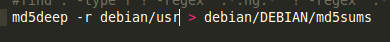
\includegraphics[width=0.6\linewidth]{md5sums}}
\caption{ Файл md5sums }
\label{md5sums:md5sums}
\end{figure}

Далее, чтобы распаковать *.deb-пакет для установки на компьютер пользователя, необходимо всем файлам задать права доступа root, иначе пакет не установится, после чего утилитой dpkg собрать из всех созданных файлов пакет формата *.deb. 

\subsubsection{Тестирование созданного пакета}

После создания *.deb-пакета для его тестирования выбраны были три образа операционных систем семейства Unix, а именно: Linux Mint 17.2, Ubuntu 14.04, Debian 8.2. На каждой из операционных систем был установлен пакет coex\_0.1-43-g59b4cc1\_all.deb. Программное обеспечение было успешно установлено, все плагины работают (рис.~\ref{debian:debian}).

\begin{figure}[h!]
\center{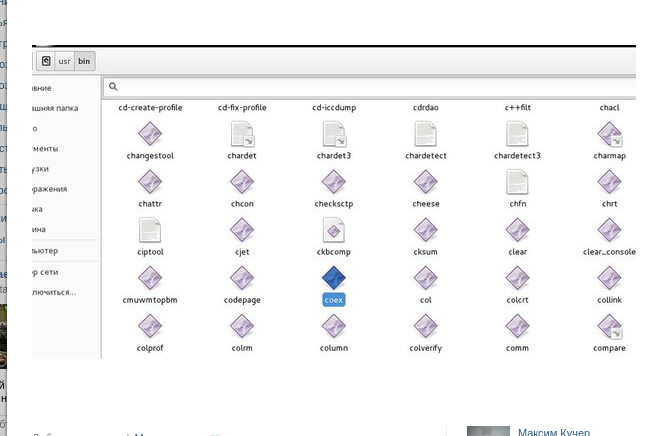
\includegraphics[width=0.8\linewidth]{debian}}
\caption{ Бинарный файл coex на debian}
\label{debian:debian}
\end{figure}

Библиотеки и исполняемые файлы плагинов coex на debian --- рисунок~\ref{debian2:debian2}.

\begin{figure}[h!]
\center{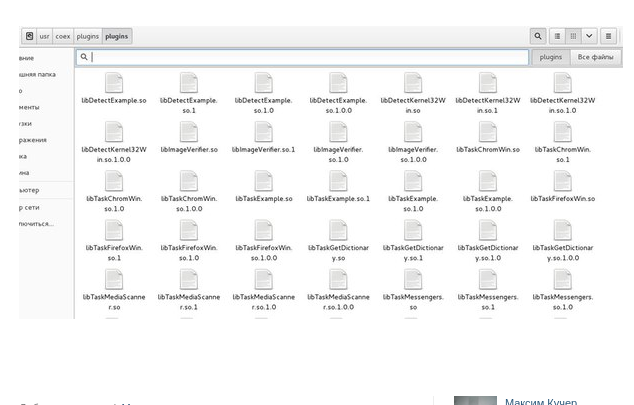
\includegraphics[width=0.9\linewidth]{debian2}}
\caption{ Библиотеки и исполняемый файлы плагинов coex на debian}
\label{debian2:debian2}
\end{figure}

Бинарный файл coex на Linux Mint --- рисунок~\ref{Linux_Mint:Linux_Mint}.

\begin{figure}[h!]
\center{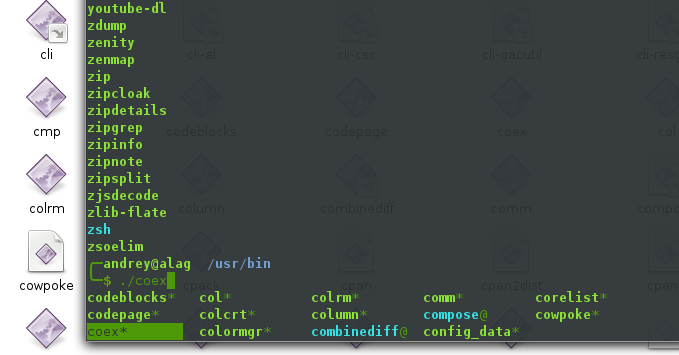
\includegraphics[width=0.6\linewidth]{Linux_Mint}}
\caption{ Бинарный файл coex на Linux Mint}
\label{Linux_Mint:Linux_Mint}
\end{figure}

Плагины на Linux Mint --- рисунок~\ref{Plugins:Plugins}.

\begin{figure}[h!]
\center{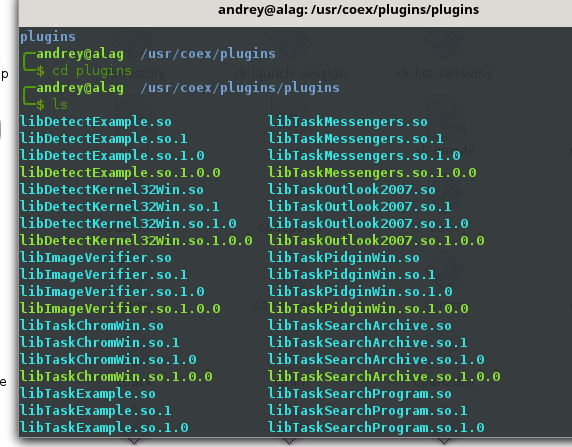
\includegraphics[width=0.6\linewidth]{Plugins}}
\caption{ Бинарный файл coex на Linux Mint}
\label{Plugins:Plugins}
\end{figure}

Запуск плагина на Linux Mint --- рисунок~\ref{Zapusk:Zapusk}.

\begin{figure}[h!]
\center{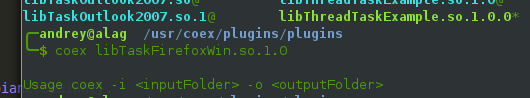
\includegraphics[width=0.6\linewidth]{Zapusk}}
\caption{ Запуск плагина на Linux Mint}
\label{Zapusk:Zapusk}
\end{figure}

Бинарный файл coex на Ubuntu --- рисунок~\ref{ubuntu:ubuntu}.

\begin{figure}[h!]
\center{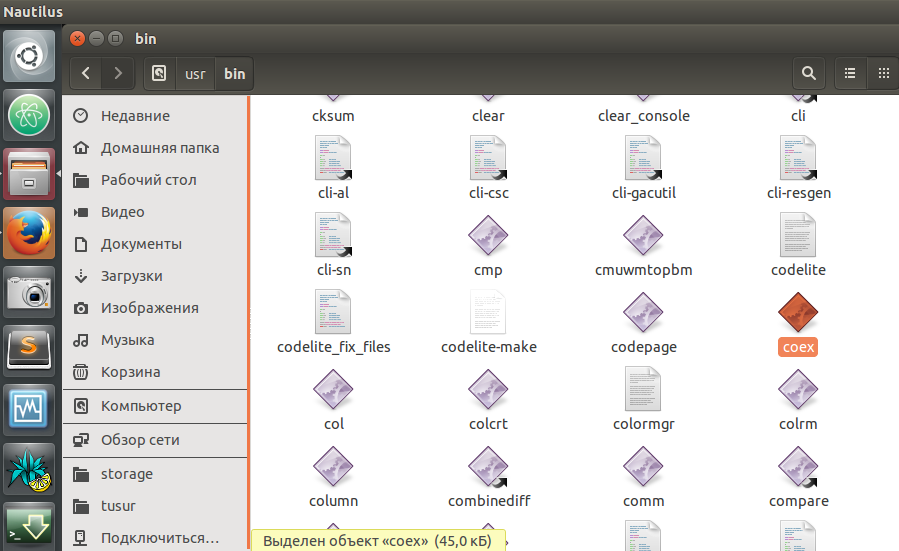
\includegraphics[width=0.8\linewidth]{ubuntu}}
\caption{ Бинарный файл coex на Ubuntu 15.04 }
\label{ubuntu:ubuntu}
\end{figure}

Запуск coex на Ubuntu --- рисунок~\ref{ubuntu2:ubuntu2}.

\begin{figure}[h!]
\center{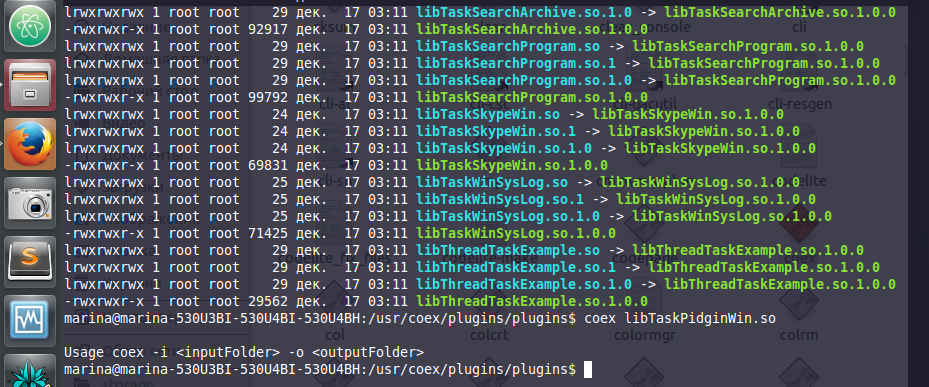
\includegraphics[width=0.8\linewidth]{ubuntu2}}
\caption{ Запуск coex на Ubuntu 15.04 }
\label{ubuntu2:ubuntu2}
\end{figure}

\clearpage







